% Hình minh họa ranh giới purge/maturity, không khẳng định ngày hoặc độ dài fold.
% Nguồn contract và hash sản phẩm được ghi trong thesis/evidence.md.
\documentclass[10pt]{article}
\usepackage[T1]{fontenc}
\usepackage{lmodern}
\usepackage[paperwidth=170mm,paperheight=118mm,margin=4mm]{geometry}
\usepackage{tikz}
\usetikzlibrary{arrows.meta}
\pagestyle{empty}
\setlength{\parindent}{0pt}
\definecolor{ink}{HTML}{1F3445}
\definecolor{good}{HTML}{126B80}
\definecolor{bad}{HTML}{B14635}
\begin{document}
\centering
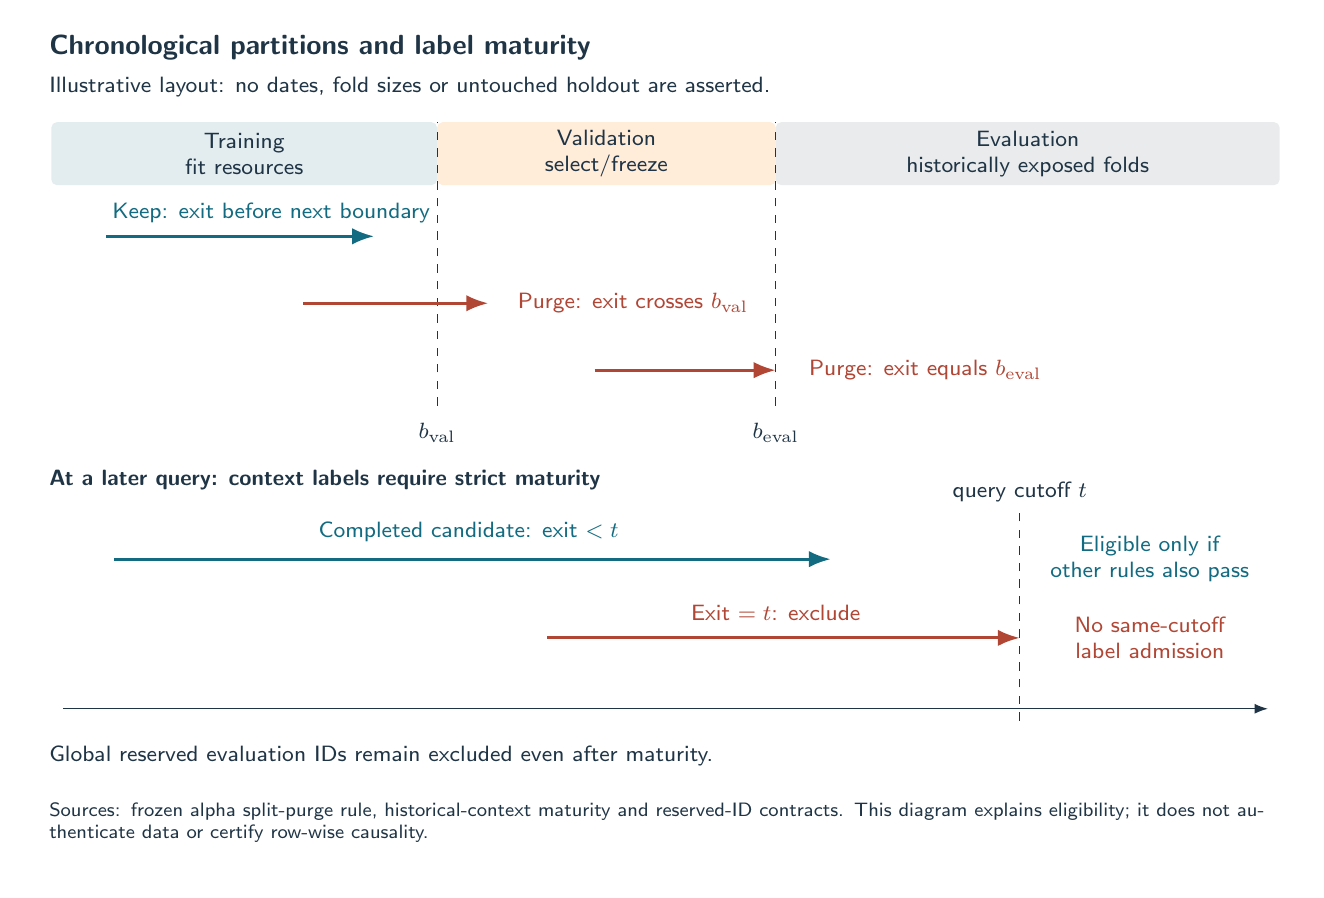
\begin{tikzpicture}[x=1cm,y=1cm,>=Latex,font=\sffamily\small,text=ink]
\path[use as bounding box] (0,0) rectangle (16.1,10.7);
\node[anchor=west,font=\sffamily\bfseries] at (.15,10.45)
  {Chronological partitions and label maturity};
\node[anchor=west,font=\sffamily\footnotesize] at (.15,9.95)
  {Illustrative layout: no dates, fold sizes or untouched holdout are asserted.};
\fill[good!12,rounded corners=2pt] (.3,8.7) rectangle (5.2,9.5);
\fill[orange!15,rounded corners=2pt] (5.2,8.7) rectangle (9.5,9.5);
\fill[ink!10,rounded corners=2pt] (9.5,8.7) rectangle (15.9,9.5);
\node[align=center,font=\sffamily\footnotesize] at (2.75,9.1)
  {Training\\fit resources};
\node[align=center,font=\sffamily\footnotesize] at (7.35,9.1)
  {Validation\\select/freeze};
\node[align=center,font=\sffamily\footnotesize] at (12.7,9.1)
  {Evaluation\\historically exposed folds};
\draw[ink,dashed] (5.2,5.9) -- (5.2,9.5);
\draw[ink,dashed] (9.5,5.9) -- (9.5,9.5);
\node[anchor=north,font=\sffamily\footnotesize] at (5.2,5.8) {$b_{\mathrm{val}}$};
\node[anchor=north,font=\sffamily\footnotesize] at (9.5,5.8) {$b_{\mathrm{eval}}$};
\draw[good,->,line width=1.1pt] (1.0,8.05) -- (4.4,8.05);
\node[anchor=west,font=\sffamily\footnotesize,text=good] at (.95,8.35)
  {Keep: exit before next boundary};
\draw[bad,->,line width=1.1pt] (3.5,7.2) -- (5.85,7.2);
\node[anchor=west,font=\sffamily\footnotesize,text=bad] at (6.1,7.2)
  {Purge: exit crosses $b_{\mathrm{val}}$};
\draw[bad,->,line width=1.1pt] (7.2,6.35) -- (9.5,6.35);
\node[anchor=west,font=\sffamily\footnotesize,text=bad] at (9.8,6.35)
  {Purge: exit equals $b_{\mathrm{eval}}$};

\node[anchor=west,font=\sffamily\bfseries\footnotesize] at (.15,4.95)
  {At a later query: context labels require strict maturity};
\draw[ink,dashed] (12.6,1.9) -- (12.6,4.55);
\node[anchor=south,font=\sffamily\footnotesize] at (12.6,4.55) {query cutoff $t$};
\draw[good,->,line width=1.1pt] (1.1,3.95) -- (10.2,3.95);
\node[anchor=south,font=\sffamily\footnotesize,text=good] at (5.6,4.05)
  {Completed candidate: exit $<t$};
\node[align=center,font=\sffamily\footnotesize,text=good] at (14.25,3.95)
  {Eligible only if\\other rules also pass};
\draw[bad,->,line width=1.1pt] (6.6,2.95) -- (12.6,2.95);
\node[anchor=south,font=\sffamily\footnotesize,text=bad] at (9.5,3.05)
  {Exit $=t$: exclude};
\node[align=center,font=\sffamily\footnotesize,text=bad] at (14.25,2.95)
  {No same-cutoff\\label admission};
\draw[ink,->] (.45,2.05) -- (15.75,2.05);
\node[anchor=west,font=\sffamily\footnotesize] at (.15,1.45)
  {Global reserved evaluation IDs remain excluded even after maturity.};
\node[anchor=west,align=left,text width=15.6cm,font=\sffamily\scriptsize] at (.15,.6)
  {Sources: frozen alpha split-purge rule, historical-context maturity and reserved-ID contracts.
   This diagram explains eligibility; it does not authenticate data or certify row-wise causality.};
\end{tikzpicture}
\end{document}
